\documentclass[a4paper,12pt]{article}
\usepackage[brazilian]{babel}
\usepackage[left=2.5cm,right=2.5cm,top=3cm,bottom=2.5cm]{geometry}
\usepackage{mathtools}
\usepackage{amsthm}
\usepackage{amsmath}
%\usepackage{nccmath}
\usepackage{amssymb}
\usepackage{amsfonts}
\usepackage{physics}
%\usepackage{dsfont}
%\usepackage{mathrsfs}

\usepackage{titling}
\usepackage{indentfirst}

\usepackage{bm}
\usepackage[dvipsnames]{xcolor}
\usepackage{cancel}

\usepackage{xurl}
\usepackage[colorlinks=true]{hyperref}

\usepackage{float}
\usepackage{graphicx}
%\usepackage{tikz}
\usepackage{caption}
\usepackage{subcaption}

%%%%%%%%%%%%%%%%%%%%%%%%%%%%%%%%%%%%%%%%%%%%%%%%%%%

\newcommand{\eps}{\epsilon}
\newcommand{\vphi}{\varphi}
\newcommand{\cte}{\text{cte}}

\newcommand{\N}{\mathbb{N}}
\newcommand{\Z}{\mathbb{Z}}
\newcommand{\Q}{\mathbb{Q}}
\newcommand{\R}{\vb{R}}
\newcommand{\C}{\mathbb{C}}
\renewcommand{\S}{\hat{S}}
%\renewcommand{\H}{\s{H}}

\renewcommand{\a}{\vb{a}}
\newcommand{\nn}{\hat{n}}
\renewcommand{\d}{\dagger}
\newcommand{\up}{\uparrow}
\newcommand{\down}{\downarrow}

\newcommand{\0}{\vb{0}}
%\newcommand{\1}{\mathds{1}}
\newcommand{\E}{\vb{E}}
\newcommand{\B}{\vb{B}}
\renewcommand{\v}{\vb{v}}
\renewcommand{\r}{\vb{r}}
\renewcommand{\k}{\vb{k}}
\newcommand{\p}{\vb{p}}
\newcommand{\q}{\vb{q}}
\newcommand{\F}{\vb{F}}

\newcommand{\s}{\sigma}
%\newcommand{\prodint}[2]{\left\langle #1 , #2 \right\rangle}
\newcommand{\cc}[1]{\overline{#1}}
\newcommand{\Eval}[3]{\eval{\left( #1 \right)}_{#2}^{#3}}

\newcommand{\unit}[1]{\; \mathrm{#1}}

\newcommand{\n}{\medskip}
\newcommand{\e}{\quad \mathrm{e} \quad}
\newcommand{\ou}{\quad \mathrm{ou} \quad}
\newcommand{\virg}{\, , \;}
\newcommand{\ptodo}{\forall \,}
\renewcommand{\implies}{\; \Rightarrow \;}
%\newcommand{\eqname}[1]{\tag*{#1}} % Tag equation with name

\setlength{\droptitle}{-7em}

\theoremstyle{plain}
\newtheorem{theorem}{Teorema}[section]
%\newtheorem{defi}[theorem]{Definição}
\newtheorem{lemma}[theorem]{Lema}
%\newtheorem{corol}[theorem]{Corolário}
%\newtheorem{prop}[theorem]{Proposição}
%\newtheorem{example}{Exemplo}
%
%\newtheorem{inneraxiom}{Axioma}
%\newenvironment{axioma}[1]
%  {\renewcommand\theinneraxiom{#1}\inneraxiom}
%  {\endinneraxiom}
%
%\newtheorem{innerpostulado}{Postulado}
%\newenvironment{postulado}[1]
%  {\renewcommand\theinnerpostulado{#1}\innerpostulado}
%  {\endinnerpostulado}
%
%\newtheorem{innerexercise}{Exercício}
%\newenvironment{exercise}[1]
%  {\renewcommand\theinnerexercise{#1}\innerexercise}
%  {\endinnerexercise}
%
%\newtheorem{innerthm}{Teorema}
%\newenvironment{teorema}[1]
%  {\renewcommand\theinnerthm{#1}\innerthm}
%  {\endinnerthm}
%
\newtheorem{innerlema}{Lema}
\newenvironment{lema}[1]
  {\renewcommand\theinnerlema{#1}\innerlema}
  {\endinnerlema}
%
%\theoremstyle{remark}
%\newtheorem*{hint}{Dica}
%\newtheorem*{notation}{Notação}
%\newtheorem*{obs}{Observação}


\title{\Huge{\textbf{Fuja do Nabo - P2}}}
\date{\vspace{-10ex}}

\begin{document}

\maketitle

\section{Questões 7-10 da P1 de 2022}

Um corpo preso na extremidade de uma mola e imerso em um
fluido viscoso, executa um movimento harmˆonico amortecido no regime subcr´ıtico conforme a equa¸c˜ao
hor´aria:
$$
x(t) = 4 e^{-3t} \cos(4t + \phi) \unit{m}.
$$
O corpo tem massa M = 1 kg e possui velocidade nula no instante de tempo t = 0 s. Sabendo que
a equa¸c˜ao diferencial deste movimento é
$$
\ddot{x} + \gamma \dot{x} + \omega_0^2x = 0.
$$
Determine:

\begin{enumerate}
\item A frequˆencia natural de oscila¸c˜ao ω0 e a constante de viscosidade ρ = γM:

\item A fase inicial ϕ do movimento:

\item O tempo necess´ario para que a amplitude m´axima do movimento se reduza `a metade do valor inicial:

\item Supondo que seja poss´ıvel variar apenas γ, qual deveria ser seu valor para o caso
do amortecimento cr´ıtico? Da mesma forma, supondo que seja poss´ıvel variar apenas ω0, qual
deveria ser seu valor para o caso do amortecimento supercr´ıtico?
\end{enumerate}

\section{Questões 1-3 da P2 de 2022}

Um bloco de massa m = 2 kg, preso a duas molas idˆenticas, com
comprimentos naturais iguais a l0 = 0,5 m e constantes el´asticas iguais a k = 400 N/m, est˜ao dentro
de um recipiente com um l´ıquido, cujo coeficiente de atrito viscoso vale ρ = 80 kg/s. Uma for¸ca
harmˆonica de amplitude F0 = 100 N e frequˆencia angular ω = 10 rad/s atua sobre o bloco ao
longo da dire¸c˜ao horizontal. O atrito entre o bloco e o fundo do recipiente ´e desprez´ıvel. Usando o
referencial da figura, determine:
\begin{figure}[H]
\centering
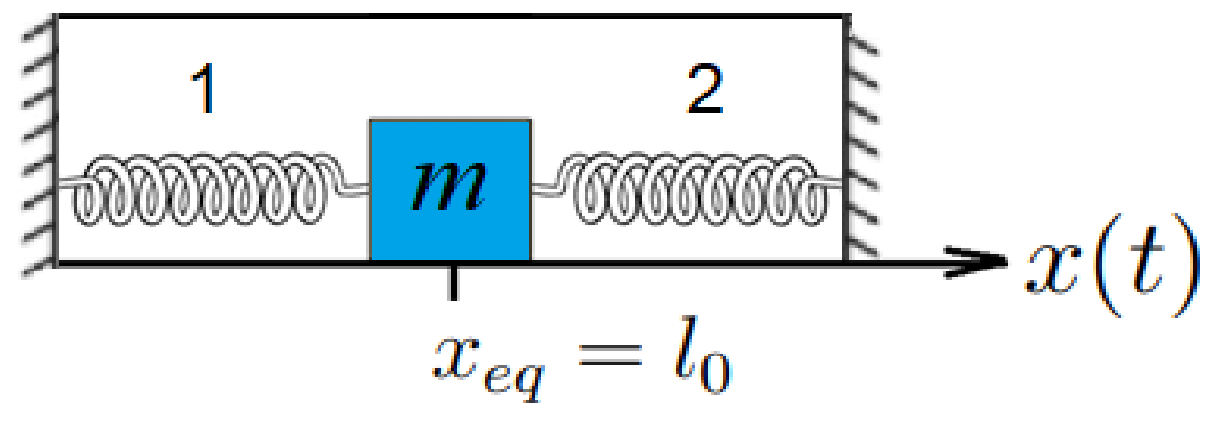
\includegraphics[width=0.6\linewidth]{fig/duas_molas.png}
\label{fig:duas_molas}
\end{figure}

\begin{enumerate}
\item A express˜ao da for¸ca el´astica que as molas exercem sobre o corpo, pode ser escrita
como:

\item A frequˆencia natural de oscila¸c˜ao, ω0, do sistema vale:

\item A solu¸c˜ao da equa¸c˜ao de movimento no regime estacion´ario, em fun¸c˜ao de t,
considerando xeq=0 m:
\end{enumerate}


\section{Questões 1-3 da REC de 2022}

O gr´afico de x(t), mostrado na figura abaixo, representa a equa¸c˜ao
hor´aria de um oscilador criticamente amortecido, para um sistema composto de um corpo de massa
m = 1, 0 kg preso a uma mola de constante el´astica k e imerso em um l´ıquido viscoso, de coeficiente
de resistˆencia viscosa ρ. A equa¸c˜ao hor´aria pode ser escrita como x(t) = e− γ
2 t(A + Bt).
\begin{figure}[H]
\centering
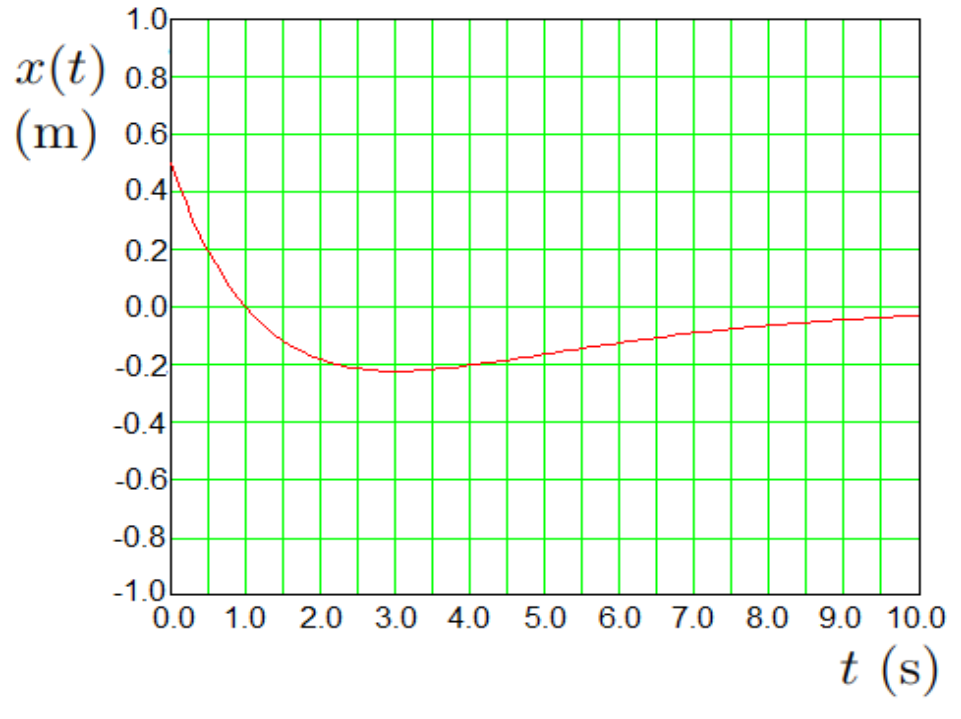
\includegraphics[width=0.6\linewidth]{fig/grafico_rec.png}
\label{fig:grafico_rec}
\end{figure}

\begin{enumerate}
\item Determine os valores de A e B.

\item Determine o coeficiente de resistˆencia viscosa ρ e a constante el´astica k da mola.

\item Determine o valor da velocidade inicial v0 do oscilador.
\end{enumerate}


\section{Questões 2-5 da SUB de 2022}

O gr´afico abaixo representa a equa¸c˜ao hor´aria x(t) de um oscilador,
para um sistema composto por um bloco de massa m = 1 kg preso a uma mola de constante el´astica
k que est´a na posi¸c˜ao horizontal. Este sistema est´a imerso em um l´ıquido viscoso com coeficiente
de resistˆencia ρ = 0, 4 Ns/m e cuja for¸ca de resistˆencia ´e proporcional `a velocidade do corpo que se
movimenta em seu interior. Dado que a velocidade inicial do bloco ´e v0 = −2 m/s, considerando o
intervalo de tempo mostrado no gr´afico, responda:

\begin{figure}[H]
\centering
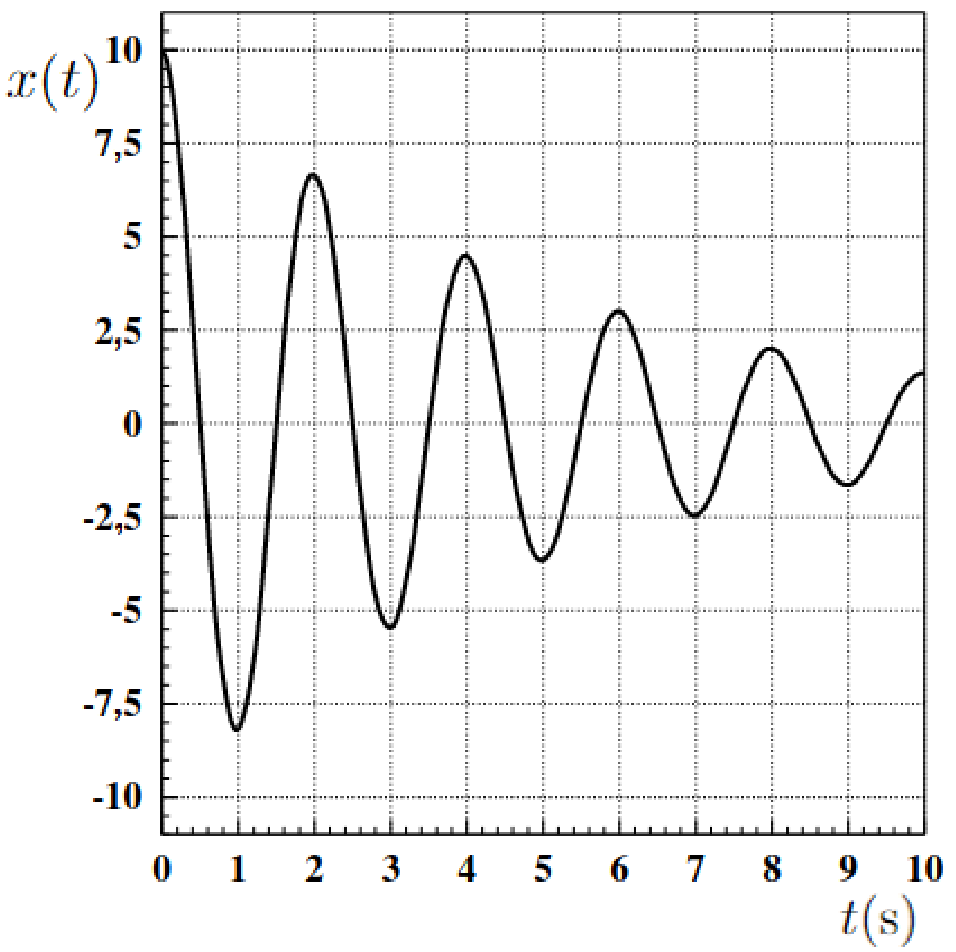
\includegraphics[width=0.6\linewidth]{fig/grafico_sub}
\label{fig:grafico_sub}
\end{figure}

\begin{enumerate}
\item Dado o movimento do bloco no sistema descrito acima, qual a equa¸c˜ao hor´aria que
descreve este sistema?

\item Determine a constante el´astica da mola k.

\item Qual a velocidade do bloco no instante t = 3 s

\item Suponha agora que este mesmo sistema seja retirado do l´ıquido viscoso e passe a
oscilar num meio sem resistˆencia. Neste novo regime, o deslocamento m´aximo ´e xmax=10 m e a
constante de fase ´e nula. Qual ser´a a nova equa¸c˜ao hor´aria do sistema?
\end{enumerate}





\end{document}
